\section{Zapis i odczyt stanu gry (Bartosz Strzelecki)}\label{s:save_impl}

Gracz w dowolnym momencie rozgrywki może przerwać grę i dokonać zapisu. Wykonuje to
za pomocą skrótu klawiszowego F8. Powoduje to zapisanie na dysk danych wszystkich obiektów posiadających
komponent "Saveable". Strukturę serlializowanych danych reprezentuje plik proto \ref{proto}.
\lstinputlisting[caption=Plik .proto reprezentujący strukturę zapisu stanu gry, label=proto]{images/game_save.proto}

Powstały po zapisie plik jest przechowywany na dysku w lokalizacji zdefiniowanej przez stałą \verb|Environment.SpecialFolder.MyDocuments| w formie binarnej (rys. \ref{save}).
W tym przypadku zapamiętywane są jedynie dane, które zmieniają się w trakcie rozgrywki, takie jak położenie gracza, przeciwników, itd. 
Zawartość statyczna taka jak krzywizna terenu i flora występująca na mapie nie jest zapisywana, a jej wczytywanie jest rozwiązywane
w trackie ładowania sceny przez Unity Runtime.

\begin{figure}[h]
\centering
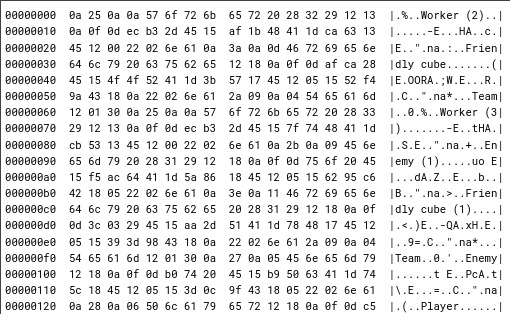
\includegraphics[width=1\textwidth]{images/save}
\caption{Zawartość przykładowego zapisu gry.}
\label{save}
\end{figure}

W momencie, w którym gracz zażąda odczytania zapisu gry, następuje proces odwrotny. Odpowiednie obiekty zostają utworzone,
a następnie przypisywane są im wartości na podstawie danych zawartych w pliku zapisu. Obiekty identyfikowane
są po ich nazwie, w taki sposób, w jaki są zarządzane przez Unity.
Tę akcję gracz wykonuję za pomocą przycisku F9 lub poprzez wybranie interesującego go zapisu z menu głównego.

